Information systems (IS) have always tried to model parts of reality. To achieve this modelling, IS contain data representing properties of real-world objects or concepts~\cite{JoseEnriquePons2012},~\cite{Billiet2012}. As time is an essential aspect of many real-world objects or concepts, IS often contain data representing temporal notions which describe such temporal properties~\cite{Bolour1982},~\cite{VanderCruyssen1997}. Such temporal notions usually take the form of either instants~\cite{Jensen1998}, which can informally be seen as infinitely short `moments' or `points' in time, or time intervals~\cite{Jensen1998}.

Data are often produced by humans, but human-made data are prone to imperfections: some data may be vague, imprecise, incomplete, contradictory or uncertain. Data representing temporal notions may contain such imprecisions too~\cite{JoseEnriquePons2012},~\cite{Billiet2012},~\cite{VanderCruyssen1997},~\cite{Devos1994},~\cite{Dubois2003}. Although The work presented in this paper is specifically concerned with time intervals (and as a special case: instants) subject to uncertainty.

Generally, one of the most important purposes of an IS is to allow the retrieval of information or knowledge deduced from its data. Such retrieval is usually done by querying the IS and examining or analyzing the query results or by visualizing the contents of the IS, querying this visualization and examining or analyzing the resulting visualization(s).

Of course, when temporal information is represented in an IS, querying this IS may have a temporal aspect too. Usually, querying such an IS is conceptually done by specifying one or more time indications and requesting information that is in a specific relationship with these indications, where the semantics of these relationships are specifically temporal~\cite{JoseEnriquePons2012},~\cite{Billiet2012},~\cite{Pons2012a}. Thus, some existing proposals have considered groups of basic relationships between time indications used to construct and express specific temporal relationships~\cite{Medina1994},~\cite{Schockaert2008},~\cite{Dubois2007}. Notably, Allen~\cite{Allen1983} presented a reasoning framework containing all semantically useful basic temporal relationships between time intervals (and as a special case instants) and subsequently used these in a framework to represent and reason with time-related actions~\cite{Allen1984} and compared them with other approaches~\cite{Allen1991}. The resulting relationships are shown in figure \ref{fig:allen-relationships}. These Allen relationships are used in the presented work.

\begin{figure}[h]
   \centering
   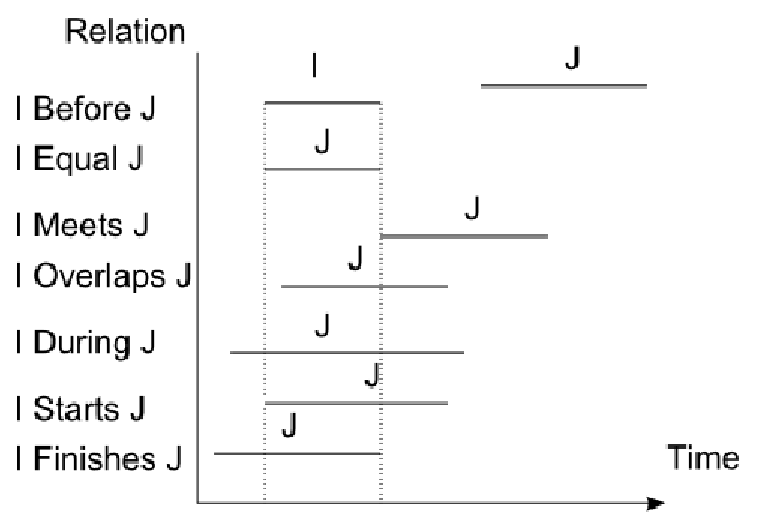
\includegraphics[width=0.9\columnwidth]{graphs/allen.eps}
   \caption{The Allen relationships between two crisp intervals $I$ and $J$.  }
   \label{fig:allen-relationships}
 \end{figure}

To be able to query IS containing data representing time indications subject to uncertainty, a framework is necessary, able to represent uncertainties in time indications in a semantically sound way, without (much) information loss and able to temporally reason with such time indications in a semantically sound and useful way~\cite{Dubois2003},~\cite{Dubois2007},~\cite{Dubois1983}. Although more proposals for such frameworks exist, the work presented in this paper focusses on just two: the \emph{ill-known constraint \emph{(IKC)} framework}~\cite{Pons2011} and the \emph{triangular model \emph{(TM)} framework}~\cite{DeTre2012}.

The work presented in this paper consists of a comparison of both frameworks, about the approaches they use to represent time intervals subject to uncertainty and to reason about the temporal relationships between such intervals and time intervals without uncertainty.

The structure of this paper is as follows: section \ref{sec:general-preliminaries} presents some general preliminaries and naming and notation conventions used in this paper. Sections \ref{sec:ikc} and \ref{sec:tm} introduce the IKC and TM frameworks respectively: both sections first introduce some specific preliminary concepts and techniques, then explain how the representation of time intervals by the framework is done and finally show how the evaluation of Allen relationships between an interval subject to uncertainty and one without uncertainty is done. In section \ref{sec:proposal}, both frameworks are compared: first their approaches to representing time intervals are compared, next their approaches to evaluating Allen relationships. Also, an example is given. Finally, section \ref{sec:conclusions} presents the principal conclusions of the presented work and some possible future work.